\documentclass[11pt]{article}

\usepackage[english]{babel}
\usepackage[utf8]{inputenc}
\usepackage{amsmath,amssymb}
\usepackage{parskip}
\usepackage{enumitem}%%%%% enumerate setting
\setenumerate{label=(\roman*),itemsep=3pt,topsep=3pt}
\usepackage{siunitx}%%% unit
\usepackage{derivative}
\usepackage{physics}
\usepackage{hyperref}
\usepackage{tikz} %%% tikz
\usepackage{pgfplots}  %%% pgf plots
\usepgfplotslibrary{fillbetween} %%% fill between
\usepackage{color}
\usetikzlibrary{decorations.pathmorphing, patterns} %%% draw springs

\usetikzlibrary{calc}  %%% sqrt calculation

\newcommand{\ee}{\mathrm{e}}

\newcommand{\id}{\mathrm{\,d}}
\newcommand{\ii}{\mathrm{i}}
\newcommand{\rp}{\mathrm{Re\,}}

\newcommand{\vi}{\mathbf{i}}
\newcommand{\vj}{\mathbf{j}}
\newcommand{\vk}{\mathbf{k}}
\newcommand{\DAG}{(\textbf{\dag})\qquad}
\newcommand{\DDAG}{(\textbf{\ddag})\qquad}

\usepackage{amssymb}
\usetikzlibrary{patterns}
\usepackage{graphicx,tipa}
\newcommand*\diff{\mathop{}\!\mathrm{d}}
\newcommand*\Diff[1]{\mathop{}\!\mathrm{d^#1}}
% Margins
\usepackage[top=2cm, left=1.5cm, right=1.5cm, bottom=2.0cm]{geometry}
% Colour table cells
%\usepackage[table]{xcolor}
\usepackage{multido}

% Get larger line spacing in table
\newcommand{\tablespace}{\\[1.25mm]}
\newcommand\Tstrut{\rule{0pt}{2.6ex}}         % = `top' strut
\newcommand\tstrut{\rule{0pt}{2.0ex}}         % = `top' strut
\newcommand\Bstrut{\rule[-0.9ex]{0pt}{0pt}}   % = `bottom' strut

\renewcommand{\familydefault}{\sfdefault} %% sans font as a default 
\DeclareSIUnit{\ft}{ft} %%%%%%% feet unit
\DeclareMathOperator{\cosec}{cosec}  %%% cosec 
%% multiple dot lines setting
\newcommand{\Pointilles}[2][2]{%
\par\nobreak
\noindent\rule{0pt}{1.5\baselineskip}% Provides a larger gap between the preceding paragrahp and the dots
\multido{}{#2}{\noindent\makebox
[\linewidth]{\rule{0pt}{#1\baselineskip}\dotfill}\\}% ...dotted lines...
\bigskip % Gap between dots and next paragraph
}

%\pgfplotsset{every axis/.append style={
%		axis x line=middle,    % put the x axis in the middle
%		axis y line=middle,    % put the y axis in the middle
%		axis line style={->}, % arrows on the axis
%		axis equal,
%	xmajorticks=false, 	 
%	ymajorticks=false,
%	unit vector ratio*=1 1 1,
%	enlarge x limits=false,
%	xlabel={$x$},
%	ylabel={$y$},
%	x label style={=at={(current axis.right of origin), anchor=north},right =0.8mm},	
%	y label style={=at={(current axis.up of origin), anchor=north},above=0.8mm}	
%}}
       %%%%%%%  axis setting
\pgfplotsset{my style/.append style={axis lines=center,
		xmajorticks=true, 	 
		ymajorticks=true,
		xlabel={$x$},
		ylabel={$y$},
		x label style={=at={(current axis.right of origin), anchor=north},right =2mm},	
		y label style={=at={(current axis.up of origin), anchor=north},above=1mm}}}
%% default setting for x-y plane


%%%%%%%%%%%%%%%%%
%     Title     %
%%%%%%%%%%%%%%%%%
%\title{Further Mechanics } 
%\author{\textbf{\Large{Mock Exam}} \\\,\\ Date: \today}
%\date{}
\begin{document}

%\maketitle 
\begin{center}
	
	\vspace*{-1.2cm}
	
	\includegraphics[scale=0.8]{schoollogo.pdf}
	
	
	\bigskip
	
	{\Huge\bf Quiz 1}
	

	
	\bigskip
	{\LARGE\bf 
		
		\begin{tabular}{l@{\hspace{1cm}}l}
			
			Grade & AS \\[0.5ex]
			
			Subject & Statistics   \\[0.5ex]
			
			Paper Name & Paper 5  \\[0.5ex]
			
			Duration & 60 minutes
			
		\end{tabular}
		
	}
	
\end{center}
\bigskip


{\LARGE\bf Student's Information}
\vspace{0.5cm}

{\LARGE
	\begin{tabular}{|p{6cm}|p{6cm}|p{2.2cm}|p{2.2cm}|}
		\hline \rule[-1ex]{0ex}{3.5ex}Name (Pinyin) & English Name & Class
		& Group
		\\ \hline \rule[-1ex]{0ex}{3.5ex} & & & \\
		\hline
	\end{tabular}
} \bigskip


{\LARGE\bf Instructions}


{\large
	
	\begin{itemize}
		
		\item Answer {\bf all} questions.
		
		\item Use a black or dark blue pen. You may use an HB pencil for
		any diagrams or graphs.
		
		\item Do {\bf not} use an erasable pen or correction fluid.
		
		\item Write your answer to each question in the space provided.
		
		\item If additional space is needed, you should use the lined page
		at the end of this booklet; the question number or numbers must be
		clearly shown.
		
		\item You should use a calculator where appropriate.
		
		\item You must show all necessary working clearly; no marks will
		be given for unsupported answers from a calculator.
		
		\item Give non-exact numerical answers correct to $3$ significant
		figures, or $1$ decimal place for angles in degrees, unless a
		different level of accuracy is specified in the question.
		
		\item {\bf You are reminded of the need for clear representation
			in your answers.}
	\end{itemize}
	
} 
\vfill 
\medskip
{\LARGE\bf Information:} 

\begin{itemize}
	
	\item The total mark for this paper is $41$. 
	
	\item The number of marks for each question or part question is
	shown in brackets [\ ].
	
\end{itemize}




 









\thispagestyle{empty} %%%% Cover without page number
\clearpage   %%% Start the page number from 1  again.
\pagenumbering{arabic}













\newpage


%%%%%%%%%%%%%%%%%%%
%%%%%%%%%%%%%%%%%%%
%   Problem     %%%
%%%%%%%%%%%%%%%%%%%
%%%%%%%%%%%%%%%%%%%
%%% Quiz 1  Representation of data %%%
%%%%%%%%%%%%%%%%%%%
%%%%%%%%%%%%%%%%%%%

\begin{enumerate}[label=\arabic*.]
	
	
	
	%%%%%%%%%%%%%%%%%%%
	%%%%%%%%%%%%%%%%%%%
	%   Problem 1   %%%
	%%%%%%%%%%%%%%%%%%%
	%%%%%%%%%%%%%%%%%%%
	%%% Q1 10/M/J/62/3 %%%
	%%%%%%%%%%%%%%%%%%%
	%%%%%%%%%%%%%%%%%%%
	
	\item The birth weights of randomsamples of $900$ babies born in country $A$ and $900$ babies born in country $B$ are illustrated in the cumulative frequency graphs. Use suitable data from these graphs to compare the central tendency and spread of the birth weights of the two sets of babies. \hfill  [6]
	
	
	\medskip
	
	
	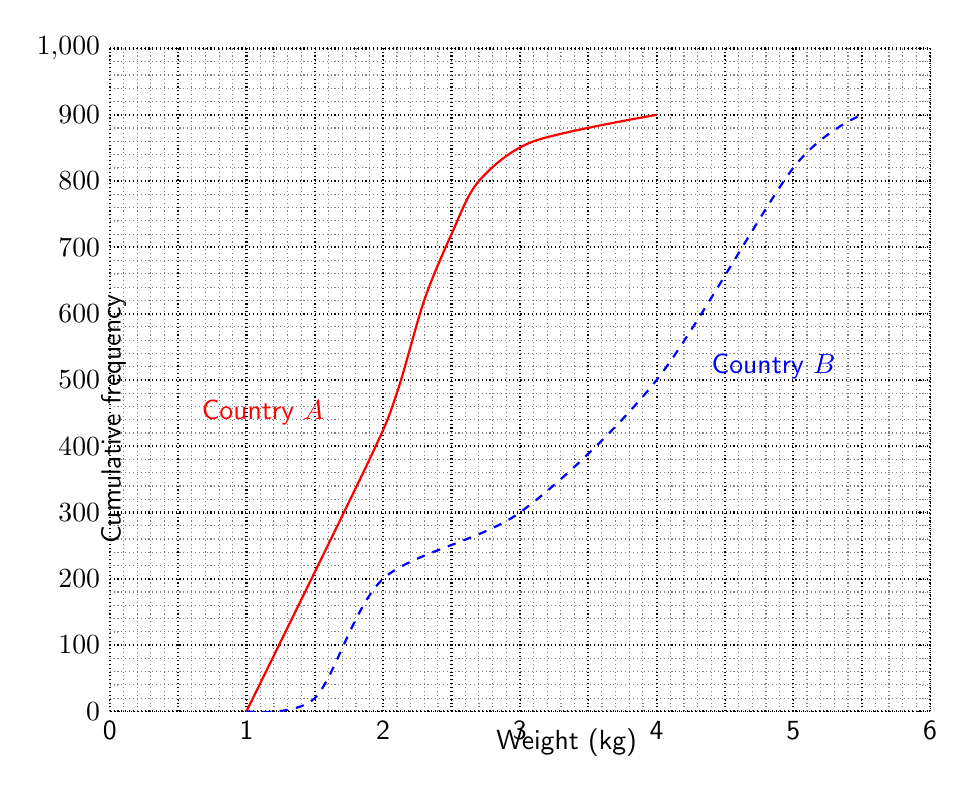
\begin{tikzpicture}
		\centering
		
		\begin{axis}[densely dotted,
			major grid style ={line width =0.8pt},
			width = 12cm,
			height = 10cm,
			%axis x line = middle,
			xmin = 0, xmax=6,
			ymin=0, ymax= 1000,
			grid = both,
			minor grid style=gray,
			ytick={0,100,200,300,400,
				500,600,700,800,900,
				1000},
			%	yticklabels={0,\empty,40,\empty,80,
			%		\empty,120,\empty,160,\empty,
			%		200
			%	},
			xtick={0,0.5,1,1.5,2,2.5,3,3.5,4,4.5,5,5.5,6},
			xticklabels={0,\empty,1,\empty,2,
			\empty,3,\empty,4,\empty,
			5,\empty,6},
			major grid style =black,
			major tick style=black,	
			minor x tick num=4,
			minor y tick num=4, 
			%extra x ticks={5,15,25,35,45,},
			%extra x tick labels={5,15,25,35,45},
			%extra y ticks={5,15,25,35,45,55},
			%extra y tick labels={\empty,\empty,\empty,\empty,\empty},
			%extra tick style={
			%	tick style=thick
			%},	
			%yticklabels={\empty,\empty,\empty},
			x label style={at={(current axis.right of origin)},anchor=north, below=0.4cm, left =3.6cm},
			y label style={at={(current axis.above origin)},anchor = west, below =0.5mm,left = 30mm},
			xlabel={Weight (kg)},
			ylabel={Cumulative frequency}
			]	
			\addplot[solid,thick, mark=none,smooth,red] plot coordinates { 
				(1,0)
				%	(2,100)
				(1.9,380)
				%	(30,600)
				(2.1,480)
				(2.3,620)
				(2.5,720)
				(2.7,800)	
				(3.1,860)
				(4,900)		
			} node[below,yshift=-3.5cm,xshift=-5cm]{Country $A$};	
			\addplot[thick, mark=none,smooth,blue,dashed] plot coordinates { 
				(1,0)
				(1.5,20)
				(2,200)
				%	(30,600)
				(3,300)
				(4,500)
				(5,820)
				(5.5,900)			
			}node[left,xshift=-0.2cm,yshift=-3.2cm]{Country $B$} ;	
			
		\end{axis}
	\end{tikzpicture}
	
	\Pointilles{10}
	
	
	
	
	
	\newpage
	
	
	%%%%%%%%%%%%%%%%%%%
	%%%%%%%%%%%%%%%%%%%
	%   Problem  2  %%%
	%%%%%%%%%%%%%%%%%%%
	%%%%%%%%%%%%%%%%%%%
	%%% Q2 11/M/J/62/3 %%%
	%%%%%%%%%%%%%%%%%%%
	%%%%%%%%%%%%%%%%%%%
	
	%% --Q2
	\item  A sample of $36$ data values, $x$, gave $\sum (x-45) = -148$ and $\sum (x-45)^2 =3089$.
	\begin{enumerate}
		\item Find the mean and standard deviation of the $36$ values. \hfill [3]
		
		\Pointilles{9}
		\item One extra data value of $29$ was added to the sample. Find the standard deviation of all $37$ values.  \hfill [4]
		\Pointilles{9}
	\end{enumerate}
	
	
	
	
	
	

\newpage
%%%%%%%%%%%%%%%%%%%
%%%%%%%%%%%%%%%%%%%
%   Problem 3   %%%
%%%%%%%%%%%%%%%%%%%
%%%%%%%%%%%%%%%%%%%
%%% Q3 09/0/N/62/6 %%%
%%%%%%%%%%%%%%%%%%%
%%%%%%%%%%%%%%%%%%%

\item The following table gives the marks, out of $75$, in a pure mathematics examination taken by $234$ students.

\begin{table}[!htpb]
	\centering
		\renewcommand{\arraystretch}{1.2} % default is 1.0
		 \setlength{\tabcolsep}{3mm}  %% set column width of a table
	\begin{tabular}{|l|c|c|c|c|c|c|}
		\hline
		Marks     & $1-20$ & $21-30$ & $31-40$ & $41-50$ & $51-60$ & $61-75$ \\ \hline
		Frequency & $40$   & $34$    & $56$    & $54$    & $29$    & $21$   \\
		\hline
	\end{tabular}
\end{table}



\begin{enumerate}
	\item Draw a histogram on graph paper to represent these results. \hfill[5]
	

	
	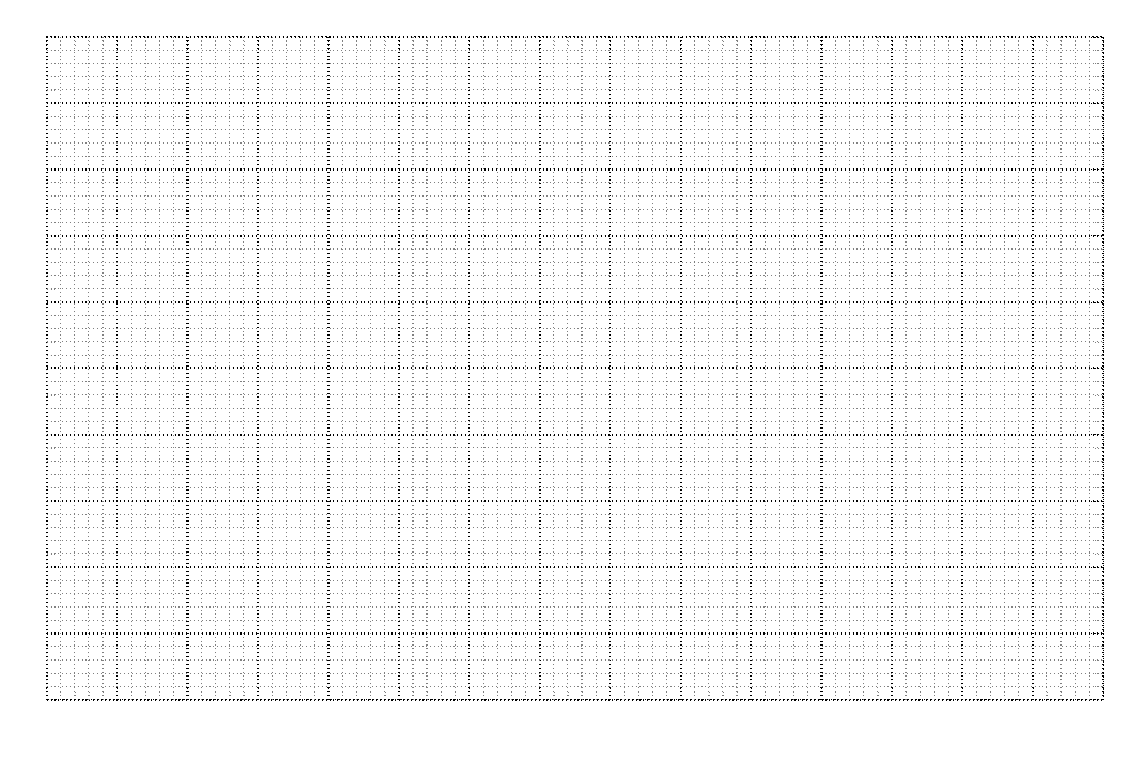
\begin{tikzpicture}
		\centering
		
		\begin{axis}[densely dotted,
			major grid style ={line width =0.8pt},
			width = 15cm,
			height = 10cm,
			%axis x line = middle,
			xmin = 0, xmax=15,
			ymin=0, ymax= 10,
			grid = both,
			minor grid style=gray,
			ytick={0,1,2,3,4,5,6,7,8,9,10,11,12},
			yticklabels={\empty,\empty,\empty,\empty,\empty,
				\empty,\empty,\empty,\empty,\empty,
				\empty,\empty,\empty
				%
			},
			xtick={0,1,2,3,4,5,6,7,8,9,10,11,12,13,14,15},
			xticklabels={\empty,\empty,\empty,\empty,\empty,
				\empty,\empty,\empty,\empty,\empty,
				\empty,\empty,\empty,\empty,\empty,
				\empty
				%
			},
			major grid style =black,
			major tick style=black,	
			minor x tick num=4,
			minor y tick num=4, 
			%extra x ticks={5,15,25,35,45,},
			%extra x tick labels={5,15,25,35,45},
			%extra y ticks={5,15,25,35,45,55},
			%extra y tick labels={\empty,\empty,\empty,\empty,\empty},
			%extra tick style={
			%	tick style=thick
			%},	
			%yticklabels={\empty,\empty,\empty},
			x label style={at={(current axis.right of origin)},anchor=north, below=0.4cm, left =3.6cm},
			y label style={at={(current axis.above origin)},anchor = west, below =0.5mm,left = 30mm},
			xlabel={\empty},
			ylabel={\empty}
			]	
			
	 		
		\end{axis}
	\end{tikzpicture}
	
	
\item  Calculate estimates of the mean mark and the standard deviation. \hfill[4]

\Pointilles{9}

\end{enumerate}

	
\newpage	
%%%%%%%%%%%%%%%%%%%
%%%%%%%%%%%%%%%%%%%
%   Problem 4   %%%
%%%%%%%%%%%%%%%%%%%
%%%%%%%%%%%%%%%%%%%
%%% Q5 14/O/N/62/6 %%%
%%%%%%%%%%%%%%%%%%%
%%%%%%%%%%%%%%%%%%%	
	
	\item  On a certain day in spring, the heights of $200$ daffodils are measured, correct to the nearest centimetre. 	The frequency distribution is given below.
	
	\begin{table}[!htpb]
			\centering
		\renewcommand{\arraystretch}{1.2} % default is 1.0
		\setlength{\tabcolsep}{2mm}  %% set column width of a table
		\begin{tabular}{|l|c|c|c|c|c|}
			\hline
			Height (cm) & $4-10$ & $11-15$ & $16-20$ & $21-25$ & $26-30$ \\ \hline
			Frequency   & $22$   & $32$    & $78$    & $40$    & $28$    \\ \hline
		\end{tabular}
	\end{table}

\begin{enumerate}
	\item Draw a cumulative frequency graph to illustrate the data.  \hfill [4]
	
		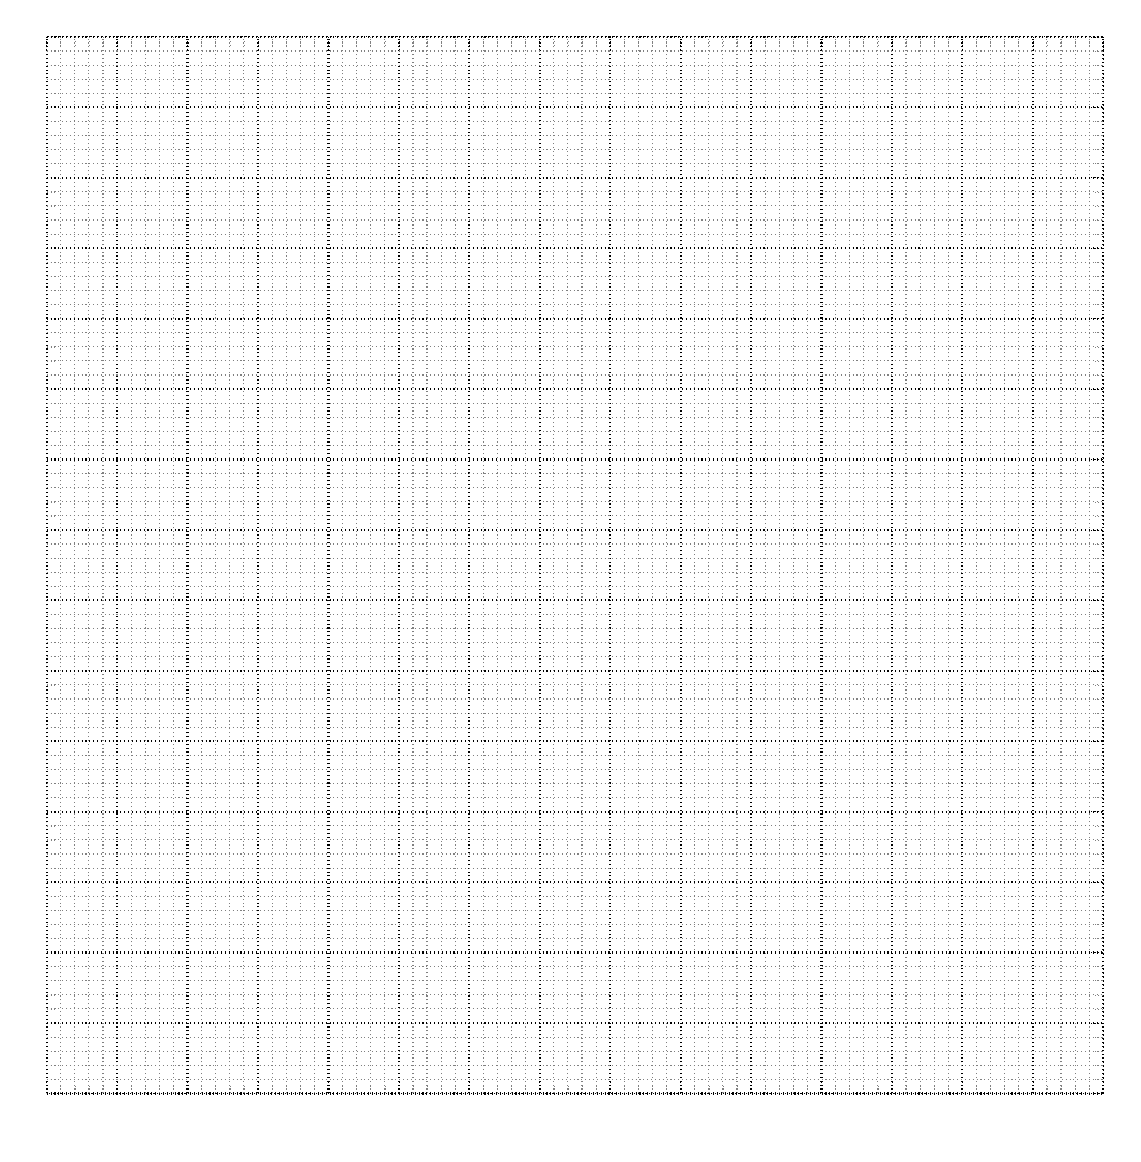
\begin{tikzpicture}
		\centering
		
		\begin{axis}[densely dotted,
			major grid style ={line width =0.8pt},
			width = 15cm,
			height = 15cm,
			%axis x line = middle,
			xmin = 0, xmax=15,
			ymin=0, ymax= 15,
			grid = both,
			minor grid style=gray,
			ytick={0,1,2,3,4,5,6,7,8,9,10,11,12,13,14,15},
			yticklabels={\empty,\empty,\empty,\empty,\empty,
				\empty,\empty,\empty,\empty,\empty,
				\empty,\empty,\empty,\empty,\empty,
				\empty
				%
			},
			xtick={0,1,2,3,4,5,6,7,8,9,10,11,12,13,14,15},
			xticklabels={\empty,\empty,\empty,\empty,\empty,
				\empty,\empty,\empty,\empty,\empty,
				\empty,\empty,\empty,\empty,\empty,
				\empty
				%
			},
			major grid style =black,
			major tick style=black,	
			minor x tick num=4,
			minor y tick num=4, 
			%extra x ticks={5,15,25,35,45,},
			%extra x tick labels={5,15,25,35,45},
			%extra y ticks={5,15,25,35,45,55},
			%extra y tick labels={\empty,\empty,\empty,\empty,\empty},
			%extra tick style={
			%	tick style=thick
			%},	
			%yticklabels={\empty,\empty,\empty},
			x label style={at={(current axis.right of origin)},anchor=north, below=0.4cm, left =3.6cm},
			y label style={at={(current axis.above origin)},anchor = west, below =0.5mm,left = 30mm},
			xlabel={\empty},
			ylabel={\empty}
			]	
			
			
		\end{axis}
	\end{tikzpicture}
	
	
	
	\item $28\%$ of these daffodils are of height $h$ cm or more. Estimate $h$. \hfill[2]
	\Pointilles{4}
	
	\item You are given that the estimate of the mean height of these daffodils, calculated from the table,	is $18.39$ cm. Calculate an estimate of the standard deviation of the heights of these daffodils. \hfill [3]
	
	\Pointilles{21}
\end{enumerate}
	
	
	
%%%%%%%%%%%%%%%%%%%
%%%%%%%%%%%%%%%%%%%
%   Problem 5   %%%
%%%%%%%%%%%%%%%%%%%
%%%%%%%%%%%%%%%%%%%
%%% Q5 10/M/J/63/6 %%%
%%%%%%%%%%%%%%%%%%%
%%%%%%%%%%%%%%%%%%%
\newpage

\item  The lengths of some insects of the same type from two countries, $X$ and $Y$, were measured. The	stem-and-leaf diagram shows the results.

\medskip

\setlength{\tabcolsep}{0.8mm}  %% set column width of a table
\begin{table}[!htpb]
	\centering
	\begin{tabular}{ccllllllllllllllllllclllllllllllllllll}
		
		\multicolumn{19}{c}{Country $X$}                                                                    &                         & \multicolumn{18}{c}{Country $Y$}                                           \\
		(10) &   &   &   &   &   &   &   &   & 9 & 7 & 6 & 6 & 6 & 4 & 4 & 4 & 3 & \multicolumn{1}{l|}{2} & \multicolumn{1}{l|}{80} &   &   &   &   &   &   &   &   &   &   &   &   &   &   &   &   &   &      \\
		(18) & 8 & 8 & 8 & 7 & 7 & 6 & 6 & 5 & 5 & 5 & 4 & 4 & 3 & 3 & 3 & 2 & 2 & \multicolumn{1}{l|}{0} & \multicolumn{1}{l|}{81} & 1 & 1 & 2 & 2 & 3 & 3 & 3 & 5 & 5 & 6 & 7 & 8 & 9 &   &   &   &   & (13) \\
		(16) &   &   & 9 & 9 & 9 & 8 & 8 & 7 & 7 & 6 & 5 & 5 & 3 & 2 & 2 & 1 & 0 & \multicolumn{1}{l|}{0} & \multicolumn{1}{l|}{82} & 0 & 0 & 1 & 2 & 3 & 3 & 3 & $q$ & 4 & 5 & 6 & 6 & 7 & 8 & 8 &   &   & (15) \\
		(16) &   &   & 8 & 7 & 6 & 5 & 5 & 5 & 3 & 3 & 2 & 2 & 2 & 1 & 1 & 1 & 0 & \multicolumn{1}{l|}{0} & \multicolumn{1}{l|}{83} & 0 & 1 & 2 & 2 & 4 & 4 & 4 & 4 & 5 & 5 & 6 & 6 & 7 & 7 & 7 & 8 & 9 & (17) \\
		(11) &   &   &   &   &   &   &   & 8 & 7 & 6 & 5 & 5 & 4 & 4 & 3 & 3 & 1 & \multicolumn{1}{l|}{1} & \multicolumn{1}{l|}{84} & 0 & 0 & 1 & 2 & 4 & 4 & 5 & 5 & 6 & 6 & 7 & 7 & 7 & 8 & 9 &   &   & (15) \\
		&   &   &   &   &   &   &   &   &   &   &   &   &   &   &   &   &   & \multicolumn{1}{l|}{}  & \multicolumn{1}{l|}{85} & 1 & 2 & $r$ & 3 & 3 & 5 & 5 & 6 & 6 & 7 & 8 & 8 &   &   &   &   &   & (12) \\
		&   &   &   &   &   &   &   &   &   &   &   &   &   &   &   &   &   & \multicolumn{1}{l|}{}  & \multicolumn{1}{l|}{86} & 0 & 1 & 2 & 2 & 3 & 5 & 5 & 5 & 8 & 9 & 9 &   &   &   &   &   &   & (11)
	\end{tabular}
	\vspace{4 pt}
	
	
	\fbox{\parbox{4.2in}{Key:  $5 |81|3$ means an insect from country $X$ has length 0.815 \si{\cm} and an insect from country $Y$ has length 0.813 \si{\cm}.}}
\end{table}
\medskip


\begin{enumerate}
	\item Find the median and interquartile range of the lengths of the insects from country $X$. \hfill [2]
	
	\Pointilles{6}
	
	\item The interquartile range of the lengths of the insects from country $Y$ is 0.028 cm. Find the values	of $q$ and $r$.  \hfill [2]
	
	\Pointilles{7}
	
	\newpage
	
	\item Represent the data by means of a pair of box-and-whisker plots in a single diagram on graph paper. \hfill [4]
	\bigskip
	
	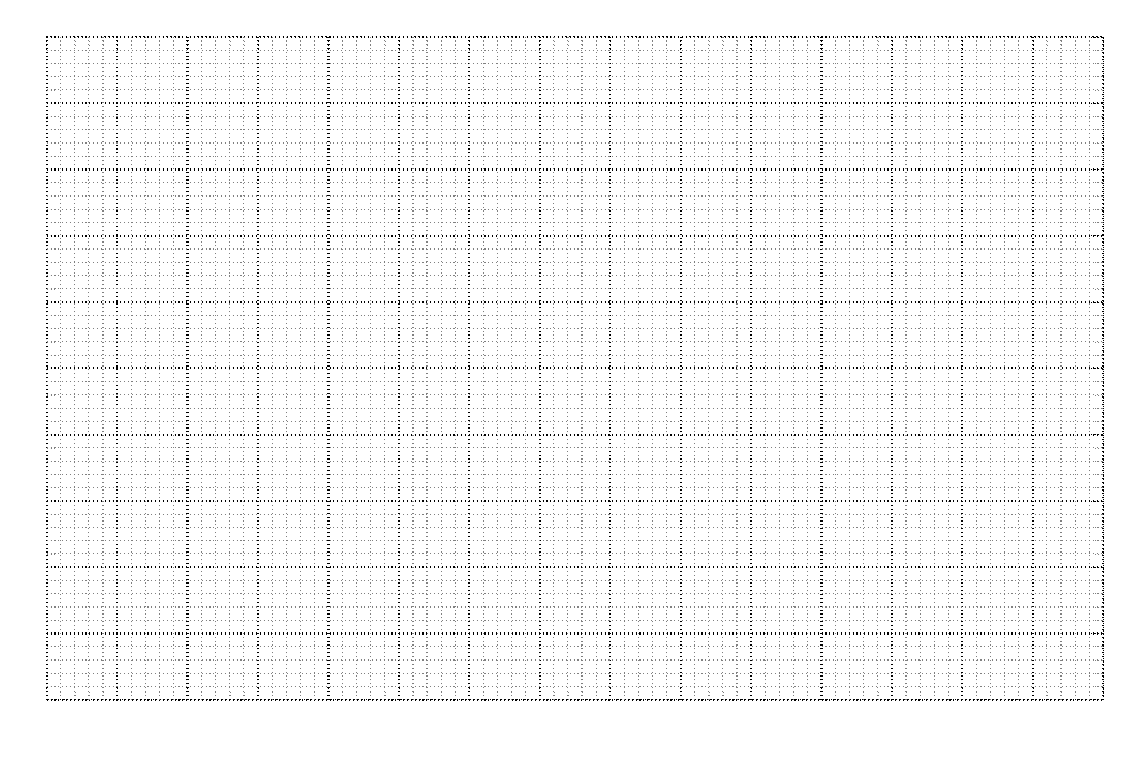
\begin{tikzpicture}
		\centering
		
		\begin{axis}[densely dotted,
			major grid style ={line width =0.8pt},
			major grid style =black,
			major grid style ={line width =0.8pt},
			%	major grid style =thick,
			major tick style=black,	
			width = 15cm,
			height = 10cm,
			%axis x line = middle,
			xmin = 0, xmax=15,
			ymin=0, ymax= 10,
			grid = both,
			minor grid style=gray,
			ytick={0,1,2,3,4,5,6,7,8,9,10,11,12},
			yticklabels={\empty,\empty,\empty,\empty,\empty,
				\empty,\empty,\empty,\empty,\empty,
				\empty,\empty,\empty
				%
			},
			xtick={0,1,2,3,4,5,6,7,8,9,10,11,12,13,14,15},
			xticklabels={\empty,\empty,\empty,\empty,\empty,
				\empty,\empty,\empty,\empty,\empty,
				\empty,\empty,\empty,\empty,\empty,
				\empty
				%
			},			
			major tick style=black,	
			minor x tick num=4,
			minor y tick num=4, 
			%extra x ticks={5,15,25,35,45,},
			%extra x tick labels={5,15,25,35,45},
			%extra y ticks={5,15,25,35,45,55},
			%extra y tick labels={\empty,\empty,\empty,\empty,\empty},
			%extra tick style={
			%	tick style=thick
			%},	
			%yticklabels={\empty,\empty,\empty},
			x label style={at={(current axis.right of origin)},anchor=north, below=0.4cm, left =3.6cm},
			y label style={at={(current axis.above origin)},anchor = west, below =0.5mm,left = 30mm},
			xlabel={\empty},
			ylabel={\empty}
			]	
			
			
		\end{axis}
	\end{tikzpicture}
	
	\bigskip
	
	
	\item Compare the lengths of the insects from the two countries. \hfill  [2]
	
	\Pointilles{10}
	
	
	
	
\end{enumerate}	
	
	

	
\end{enumerate}
\vfill

















$\cdots\cdots\cdots\cdots\cdots\cdots\cdots\cdots\cdots\cdots\cdots\cdots\cdots\cdots\cdots\cdots$  THE END $\cdots\cdots\cdots\cdots\cdots\cdots\cdots\cdots\cdots\cdots\cdots\cdots\cdots\cdots\cdots\cdots\cdots\cdots\cdots\cdots$
%\newpage
%\begin{center} 
	%\LARGE BLANK PAGE
%\end{center}

\end{document}
